\section{Gameplay}

The goal of the game is finish all the tracks on the progression map. To finish a track the player must survive several waves of mobs that try to escape land and jump into the ocean. Each time a mob reaches the ocean the player loses a life. If the player's total life reaches zero, the track is lost. To prevent this from happening the player must build towers that shoot at the mobs.

\subsection{Progression map}

The progression map visualizes the player's progress in the game and lets him choose which track he wants to play. The progression map resembles a geographical map where each track is a geographical site placed along a route. The progress map is customized to match the theme of the game. In Eskimo Tower Defense it depicts a route from the North Pole to The Sun.

The progression route is a fixed route that dictates in what order the tracks must be completed by the player. The route is visualized on the track progression map. Each track in the game is placed somewhere along the route. To be able to play a certain track, the player must first complete any tracks before it. The route may be forked, in which case only one way leading to a track needs to be cleared in order to play that track. 

The player's current progression is visualized with icons. A green icon indicates that the track has been completed. A blue icon indicates that the track is not yet completed, but available to play. A red icon indicates that the track is not yet unlocked. There are currently five tracks called: "North Pole", "Ice Flow", "I see green", "Almost there" and "The sun".  

If the player touches one of the tracks, a blue water splash is displayed on top of that track to indicate that it was selected. A menu including the name and current highscore for that track is also displayed. It will offer the options "Start Level" and "Cancel" (figure ~\ref{fig:progressionMap}).

%------------------------------
%- Image of the progression map
%------------------------------
\begin{figure}[here]

\begin{center}
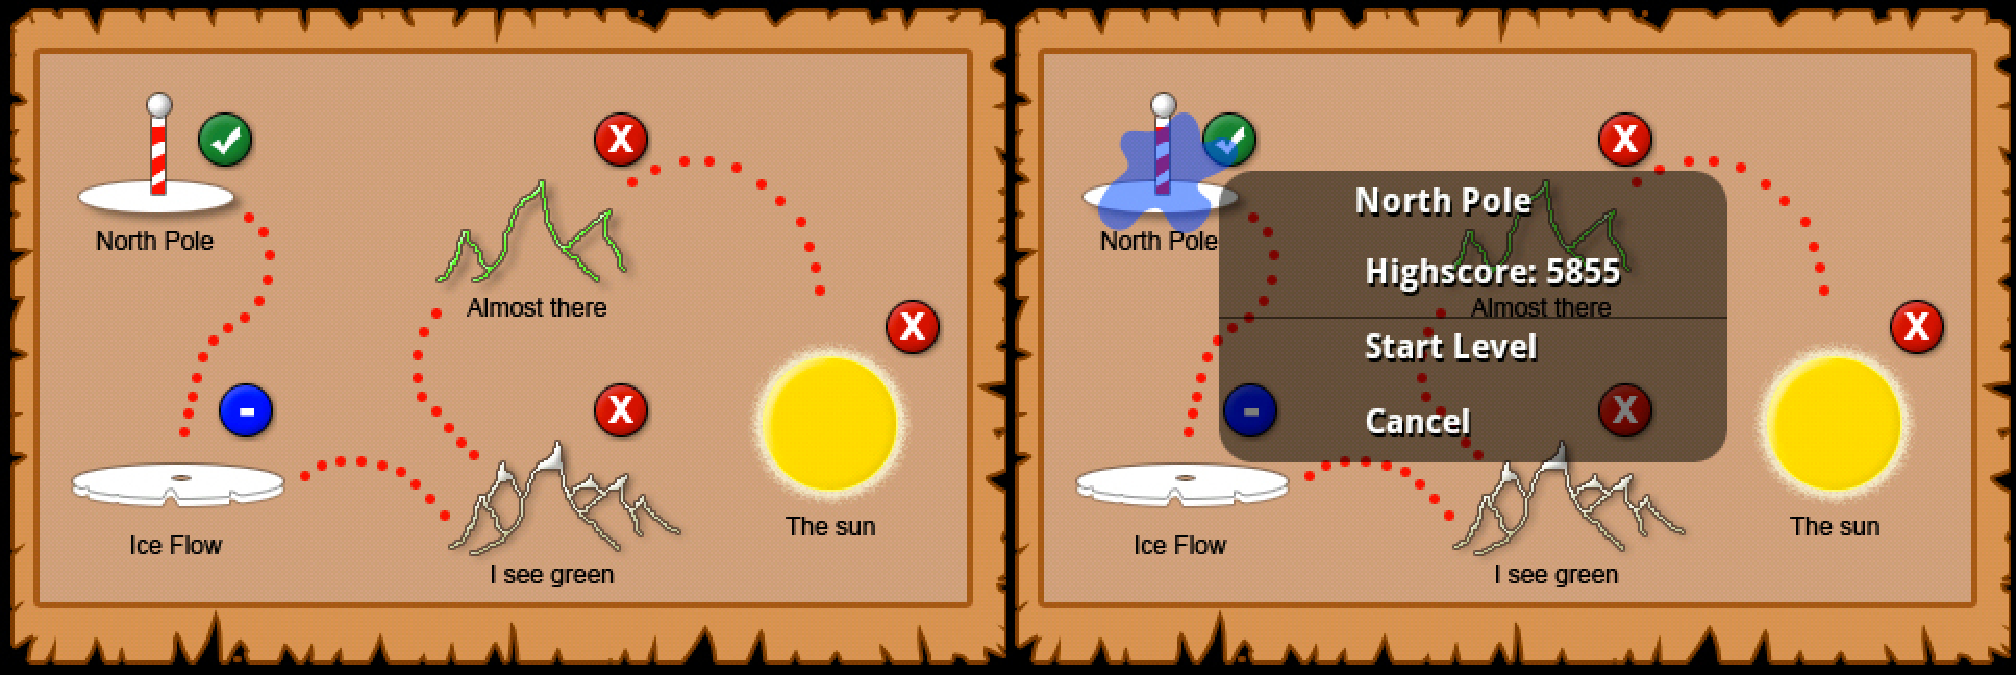
\includegraphics[scale=0.4]{pics/chapters/chapter4/progmapboth}
\end{center}

\caption{The progression map}
\label{fig:progressionMap}

\end{figure}
%------------------------------
\subsection{Game field}

Once a track is started from the progression map, the game field is shown. A background for the specified track is displayed. The player is given some time to accustomize himself to the interface, and start building towers before the first wave of mobs enter the game field.

%-------------------------
%- Image of the game field
%-------------------------
\begin{figure}[here]

\begin{center}
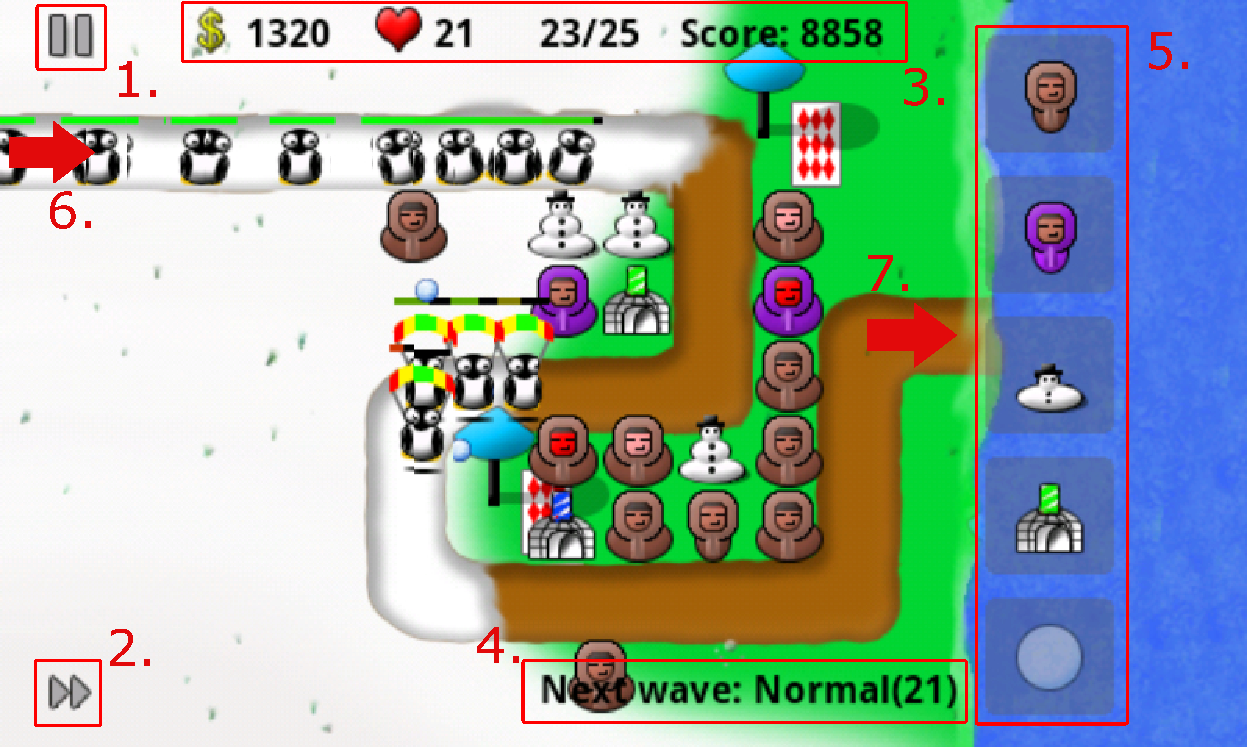
\includegraphics[scale=0.5]{pics/chapters/chapter4/thegame}
\end{center}

\caption{The game field}
\label{fig:gameField}

\end{figure}
%-------------------------

\clearpage

Figure ~\ref{fig:gameField} shows a screenshot of the game field. Points of interest are marked with numbers: \\*
{\bf 1.} The pause button: Pauses the game. \\*
{\bf 2.} Fast forward button: Triples the speed of the game. \\*
{\bf 3.} Player statistics: Money, number of lives, wave number and score. \\*
{\bf 4.} Countdown for the next wave of mobs. Includes mob type. \\*
{\bf 5.} Buttons for buying new towers. Towers are dragged to the game field. \\*
{\bf 6.} First checkpoint for new mobs. \\*
{\bf 7.} Last checkpoint for mobs on the game field.

\subsection{Mobs}

The word mob is short for mobile and is traditionally used to describe hostile units in video games \citep{netGames}. In Tower Defense games the mobs are the units that try to cross the game field.

In Eskimo Tower Defense, the mob types are distinguished graphically as different types of cold-weather animals. Each mob type has some unique characteristics. In the current implementation of the game there are five mob types:

\begin{itemize}
\item {\bf Normal:} A standard type of mob with no special features.
\item {\bf Healthy:} A boss that always comes alone and has more health, making it difficult to kill. They move slower than normal mobs, but are resistant to slowing towers, meaning they are only partly affected by slowing effects.
\item {\bf Fast:} Moves faster than normal mobs. Slowing towers can be used to decrease their speed.
\item {\bf Immune:} Are immune to the slow effect caused by slowing towers.
\item {\bf Air:} A mob type that flies. Splash towers can not damage them at all and basic towers inflict reduced damage to them. Air towers are the most effective weapon against them.
\end{itemize}
The mobs enter the game field in waves. A wave consists of one or more mobs. All the mobs in one wave are of the same mob type. The mobs enter the game one by one and walk along the path in a line. When the last mob of a wave has entered the game field, there is a small delay before the next wave arrives.

The maximum health of the mobs is increased for each wave. It is up to the player to build towers that kill the mobs before they reach the ocean. If a mob reaches the ocean, the player loses one life.

\subsection{Towers}

Towers are immobile units that the player can build and upgrade for in-game money. By shooting projectiles, they try to stop mobs from reaching the ocean. In Eskimo Tower Defense, the towers are graphically represented by two different Eskimos, a snowman and an igloo. 

The different tower types are:
\begin{itemize}
\item {\bf Basic tower:} A standard tower type with good range and damage
\item {\bf Splash tower:} A tower type with slow fire rate and small range. It shoots a projectile that hits the ground and causes damage to all mobs within its blast radius.
\item {\bf Slowing tower:} This tower type is used to slow mobs down temporarily. Its range is fairly small compared to the other towers. It will not shoot at mobs that are already slowed.
\item {\bf Air tower:} With big range and damage, this tower type is only able to shoot flying mobs.
\end{itemize}

Upgrading a tower increases its power in various ways. In some cases, this is more effective than buying new towers. 

\subsection{Projectiles}

Towers inflict damage by launching projectiles toward the mobs. Each tower type has a corresponding type of projectile with specific characteristics. 

The projectile types are:
\begin{itemize}
\item {\bf Basic projectile:} Launched by basic towers. This projectile simply inflicts damage to its target mob without any side effects.
\item {\bf Slowing projectile:} Launched by slowing towers. Apart from inflicting a small amount of damage to its target, this projectile also causes a slowing effect when reaching its target. Some mobs are affected less by this effect, some are even immune to it.
\item {\bf Splash projectile:} Launched by splash towers. It lands on the ground where the target mob was at the time of launch. When hitting the ground, it explodes and inflicts damage to all nearby mobs. 
\item {\bf Air projectile:} Launched by air towers. This works exactly like a basic projectile, except it is only shot at flying mobs.
\end{itemize}

Basic, slowing and air projectiles all lock on to their target mob, changing direction when the mob moves. Because of this, these projectiles always hit their target. The splash projectile does not lock to a target, and there is a risk that it will not hit any targets at all.

\subsection{Snowball}

Several new game mechanics are made possible by accessing the accelerometer. Eskimo Tower Defense features the ability to create a snowball that is controlled by the accelerometer sensor. The snowball is modeled to emulate a real-world snowball, which moves according to the laws of physics. Leaning the mobile device in one direction causes the snowball to accelerate in that direction. When the snowball rolls over mobs on the game field, they take damage equal to \begin{math}7\%\end{math} of their current health.

Like a real-world snowball, the in-game snowball also melts. This happens slowly over time, and also when the snowball runs over mobs. The more it melts the smaller it gets, eventually disappearing completely.

The player gains access to snowballs depending on his current score. Every time 4000 points have been added to the score, an additional snowball is available. This results in the player being able to use the snowball two to three times per track. No cost is withdrawn when a snowball is used, the snowball is meant to be a reward with no negative side effects.